\documentclass[14pt, oneside]{article}     	% use "amsart" instead of "article" for AMSLaTeX format
\usepackage{geometry}                		% See geometry.pdf to learn the layout options. There are lots.
\usepackage[dvipdfmx]{hyperref}
\usepackage{here}

\geometry{left=25mm,right=25mm,top=30mm,bottom=30mm}
\geometry{letterpaper}                   		% ... or a4paper or a5paper or ...
%\geometry{landscape}                		% Activate for rotated page geometry
%\usepackage[parfill]{parskip}    		% Activate to begin paragraphs with an empty line rather than an indent
\usepackage[dvipdfmx]{graphicx}				% Use pdf, png, jpg, or eps§ with pdflatex; use eps in DVI mode
								% TeX will automatically convert eps --> pdf in pdflatex
\usepackage{amssymb}

\usepackage{listings}
\renewcommand{\lstlistingname}{コード}
%SetFonts
\lstset{%
  language={Python},
  basicstyle={\small},%
  identifierstyle={\small},%
  commentstyle={\small\itshape},%
  keywordstyle={\small\bfseries},%
  ndkeywordstyle={\small},%
  stringstyle={\small\ttfamily},
  frame={single},
  breaklines=true,
  columns=[l]{fullflexible},%
  numbers=left,%
  xrightmargin=0zw,%
  xleftmargin=3zw,%
  numberstyle={\scriptsize},%
  stepnumber=1,
  numbersep=1zw,%
  lineskip=-0.5ex%
}
%SetFonts

\title{並列分散処理  最終レポート}
\author{チームE 大城 慶知 眞榮城 隆守 伊波卓浩 宮良友也}
%\date{}							% Activate to display a given date or no date

\begin{document}
\maketitle

\section*{最終報告書に載せるやつ(あとで消すやつ)}

演習の背景、目的、方法、結果、考察をA410ページ以内で適切にまとめる。
個々のメンバーの役割分担を明記する。記載がない場合、あるいは、曖昧な場合には、
減点の対象となる。例えば、あるタスクを複数名で担当した場合でも、個々のメンバーの
役割をできる限り区別して説明する。
最終報告書にはソースコードのgithubリポジトリも記載する。

\section{演習の背景}
「講義で説明した並列分散処理を実践し、他者に有益な情報となるように共有せよ。」という課題が渡された。

b3前期はメンバーが忙しく時間も取れないので軽量かつ有益な情報をということで、
GPUマシンを使った並列処理を断腸の思いで断念し、Pythonにおける非同期処理を用いたI/Oの並列処理を行うことにした。

\section{目的}
Pythonのスレッドとconcurrentを用いて並列化を行うとともに、
async awaitの使うことで非同期処理を行いさらに速度向上を目指す。


\section{Pythonの事前知識}

\subsection{スレッドの制約}
Pythonでは、GIL(Global Interpreter Lock)と呼ばれる制約がある。
GILとは、Figure \ref{multithred_iobound}と Figure\ref{multithred_cpubound}のように、CPUバウンドでPythonを実行した際に一つだけしかスレッドのリソースを起動できない制約である。
そのため、PythonのCPUバウンドの並列処理はプロセスを使って、I/Oバウンドの並列処理はスレッドを行う事が多い。

\begin{figure}[H]
  \centering
  \includegraphics[width=12cm]{multithred_iobound.png}
  \caption{マルチスレッドI/Oバウンド}
  \label{multithred_iobound}
\end{figure}

\begin{figure}[H]
  \centering
  \includegraphics[width=12cm]{multithred_cpubound.png}
  \caption{マルチスレッドCPUバウンド}
  \label{multithred_cpubound}
\end{figure}


\subsection{asyncとawait}
asyncとawaitがどのような処理を行うのか以下のコードを実行して動作を確認した。
\lstinputlisting[caption=非同期処理のFizzBuzz,label=FizzBuzz]{../FizzBazz/FizzBazz.py}

\begin{lstlisting}[caption=FizzBuzz実行結果]
75219:6:Fizz
8282:6:Fizz
57464:6:Fizz
75220:6:Fizz
8283:6:Fizz
57465:6:Fizz
75221:6:Fizz
8284:6:Fizz
57466:6:Fizz
75222:6:Fizz
8285:6:Fizz
57467:6:Fizz
75223:6:Fizz
\end{lstlisting}

実行結果からFizzBuzzのコードをスリープさせているのにもかかわらず、



\section{実験方法}

HTTPのGETを用いて実験を行った。
GETを複数回実行する場合を考えると、
逐次処理の場合ではレスポンスがあるまで
次のGETを送信することができない。
これを並列処理により
レスポンスを待つことなく
次のGETを実行した。
これにより効率よく
GETを実行し、
結果を受け取ることができると
想定した。

\lstinputlisting[caption=逐次処理,label=example1]{../HttpRequest/example1.py}

\lstinputlisting[caption=async-awaitのみ,label=example2]{../HttpRequest/example2.py}

\lstinputlisting[caption=async-awaitのみ(5回ずつ),label=example3]{../HttpRequest/example3.py}

\lstinputlisting[caption=async-await + MultiPoolExector,label=example4]{../HttpRequest/example4.py}

\section{実行結果}

example1.pyは逐次処理をしてくれる
スクリプト。\\
example2.pyはコルーチンを
20個一気に呼び出す。\\
example3.pyはコルーチンを
5個ずつ4回呼び出している。\\
example4.pyはスレッドを使用。\\


実行結果を以下に示す。

\lstinputlisting[caption=example1.py,label=1]{../HttpRequest/sequentially}

\lstinputlisting[caption=example2.py,label=2]{../HttpRequest/async_await20}

\lstinputlisting[caption=example3.py,label=3]{../HttpRequest/async_await5}

\lstinputlisting[caption=example4.py,label=4]{../HttpRequest/thread}

\begin{figure}[H]
  \centering
  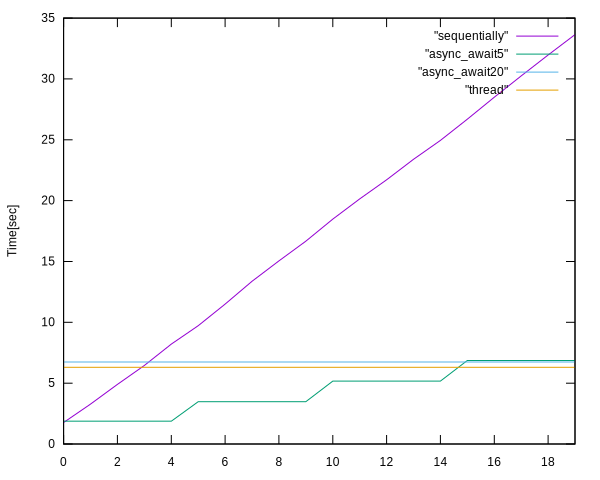
\includegraphics[width=13cm]{time.png}
  \caption{実行結果}
\end{figure}

こうなりました。


\section{考察}



\section{感想・意見}
\section*{GitHubのURL}

\subsection*{https://github.com/e165719/ParallelDistributedProcessing}

\end{document}
